\section{tasks::findord Class Reference}
\label{classtasks_1_1findord}\index{tasks::findord@{tasks::findord}}
Inheritance diagram for tasks::findord::\begin{figure}[H]
\begin{center}
\leavevmode
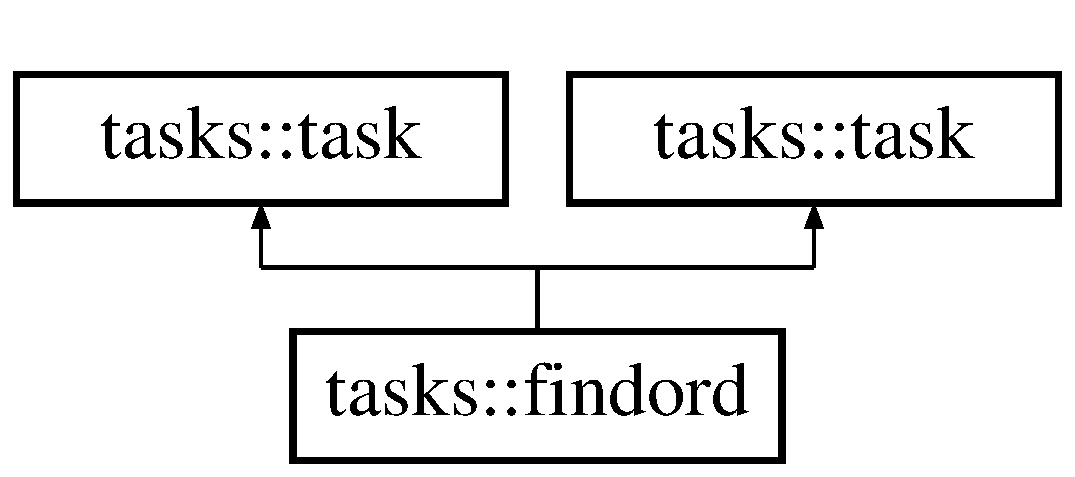
\includegraphics[height=2cm]{classtasks_1_1findord}
\end{center}
\end{figure}
\subsection*{Public Member Functions}
\begin{CompactItemize}
\item 
def \textbf{run}\label{classtasks_1_1findord_c3bc59827b3a103e304b1d2959296922}

\item 
def \textbf{run}\label{classtasks_1_1findord_c3bc59827b3a103e304b1d2959296922}

\end{CompactItemize}
\subsection*{Static Public Attributes}
\begin{CompactItemize}
\item 
string \textbf{name} = '{\bffindord}'\label{classtasks_1_1findord_f797d3fbbf58f8e94ef934c59ec7bc7c}

\item 
string \textbf{button\-Text} = 'Find order locations'\label{classtasks_1_1findord_9564a941d92e9a18c30bc7e5b3bf71c2}

\item 
int \textbf{inthread} = 0\label{classtasks_1_1findord_8dda8a8044b3c1806c5ae86930f977f9}

\end{CompactItemize}


\subsection{Detailed Description}


\footnotesize\begin{verbatim}Interactively define and trace the location of spectral orders using a well-exposed
   order-definition frame. 
\end{verbatim}
\normalsize
 



The documentation for this class was generated from the following files:\begin{CompactItemize}
\item 
old/PANICtool-1.0/tasks.py\item 
old/tasks.py\end{CompactItemize}
